\section{Information Theory}%
\label{sec:information-theory}

\vspace{1cm}

\begin{figure}[h!]%
  \label{fig:info}
  \centering
  \fcolorbox{black}{white}{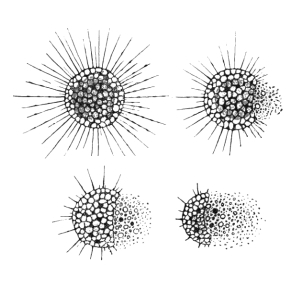
\includegraphics[width=0.3\textwidth]{entropy}}
  \caption{\href{https://www.consciousentities.com/2017/02/consciousness-entropy/}{Conscious
      Entities, Peter Hankins}}
\end{figure}

\vspace{1cm}

\noindent Information theory was born in 1948 with the publication of \textit{A
  Mathematical Theory of Communication} by Claude Shannon
(1916~\textendash~2001). Shannon was inspired in part by earlier work by
Boltzmann and Gibbs in thermodynamics and by Hartley and Nyquist at Bell,
see~\cite{ref:losee-1997}. Most of the theory and applications of information
theory (compression, coding schemes, data transfer over noisy channels) are
outside the scope of this thesis, but there are certain information theoretic
quantities used regularly in machine learning, so it is useful to discuss them
now.

\begin{remark}
  The information we talk about is restricted to the information about the
  probability distribution over the elementary outcomes, not information about
  the content of the outcomes. The significance of probability is that it tells
  us how certain we can be when making inference. The most important information
  in this regard is found in the probability distribution over the possible
  outcomes.
\end{remark}

Information theory is quite useful for deep learning. If we think of neural nets
as noisy channels, the need for this theory becomes even more obvious.
In~\cite{ref:mackay-2003}, David Mackay said ``brains are the ultimate
compression and communication systems. And the state-of-the-art algorithms for
both data compression and error-correcting codes use the same tools as machine
learning''. Furthermore, ``we might anticipate that the best data compression
algorithms will result from the development of artificial intelligence
methods''.

The most fundamental quantity in information theory is entropy. Before we state
the formal definition of entropy, we will motivate it as a measure of
uncertainty by walking through its derivation. We will define a function $\eta$
as a measure of uncertainty and we will derive entropy as a function based on
the requirements it must satisfy using $\eta$ as a starting point.

\begin{definition}
  Let $(\&X, p)$ be a discrete probability space. We define
  \textnormal{\sffamily uncertainty} to be a real-valued function
  $\eta(\cdot): \&X \mapsto \R^+$ which depends only on the
  probabilities of the elementary outcomes and satisfies the
  following:
  \begin{enumerate}[(i)]
  \item If an outcome $x$ is guaranteed to occur, then there is no
    uncertainty about it and $\eta(x) = 0$;
  \item For any two outcomes $x$, $x^\prime$, we have $p(x) < p(x^\prime) \iff
    \eta(x) > \eta(x^\prime)$;
  \item For any two independent outcomes, $x$, $x^\prime$, the
    uncertainty of their joint occurrence, is the sum of their
    uncertainties, i.e.
    $\eta(x \cdot x^\prime) = \eta(x) + \eta(x^\prime)$.
  \end{enumerate}
\end{definition}
\begin{remark}
  This definition is a modification of one given
  by~\cite{ref:martin-2011}.
\end{remark}

It should not be a surprise that it is new information we are interested in,
since that is what reduces uncertainty. Common outcomes provide less information
than rare outcomes, which means $\eta$ should be inversely proportional to the
probability of the outcome.
\begin{align}
  \label{eq:eta-1}
  \eta(x) \propto {1 \over p(x)}
\end{align}
Since $\eta$ must satisfy $\eta(x \cdot x^\prime) = \eta(x) + \eta(x^\prime)$,
we must define $\eta$ in terms of the logarithm. This is because the probability
of two independent outcomes is the product of their probabilities whereas we
want information to be additive.  Thus,
\begin{align}
  \label{eq:eta-3}
  \eta(x) \approx \log{1 \over p(x)}.
\end{align}
For probability distributions, we need a measure of uncertainty that says, on
average, how much uncertainty is contained in $(\&X, p)$. We need to weight the
calculation by the probability of observing each outcome. This means what we are
really seeking is a measure on the probability distribution over $\&X$. We
adjust the notation, using the capital eta, which resembles the Latin H. Thus,
\begin{align}
  \label{eq:eta-almost}
  \&H(p) = \sum_{x \in \&X} p(x) \log{1 \over p(x)}.
\end{align}
This is what we will call entropy, a measure on the average amount of surprise
associated to outcomes from $(\&X, p)$. Entropy is maximized when we cannot say
with any confidence if an outcome will occur. This upper bound occurs when the
probabilities over the set of possible outcomes are uniformly distributed.
\begin{align}
  \label{eq:eta-2}
  \&H(p) \leq \log{|\&X|}
\end{align}
We can also think of entropy as how much information, measured in binary
information units (bits), is required to describe outcomes drawn from $(\&X,
p)$. The way to understand this last part is the logarithm tells us how many
bits we need to describe this uncertainty, since
\begin{align}
  \label{eq:understand-log}
  \log_2{1 \over p(x)} = n \iff 2^n = {1 \over p(x)}.
\end{align}
However, any logarithm can be used. Base $e$ and base 10 are also commonly used.
\begin{definition}
  Let $(\&X, p)$ be any discrete probability space. The \textnormal{\sffamily
    entropy} of a probability distribution $p$ with mass function $p$, denoted
  by $\&H(p)$, is the average amount of uncertainty found in elementary outcomes
  from $(\&X, p)$. We write
  \begin{align}
    \label{eq:entropy}
    \&H(p) = - \mathbb{E}_{x \sim p} \left[ \log{p(x)} \right].
  \end{align}
  The entropy of a probability distribution tells us how much
  variation we should expect to see in samples drawn from $(\&X,
  p)$. The probability distribution with maximum entropy is the
  uniform distribution since all outcomes are equally surprising.
\end{definition}

Figure~\ref{fig:entropy-coin-toss} depicts the entropy of a
probability distribution over two states as a function of the symmetry
of the distribution.  As the probability of heads $p(H)$ approaches 0
or 1, we see the uncertainty vanishes, and uncertainty is maximized
when probability is equally distributed over heads and tails.

\begin{figure}[H]
  \centering
  \begin{tikzpicture}
    \begin{axis}[
      ymin = 0,
      ymax = 1,
      xmin = 0,
      xmax = 1,
      xlabel = $p(H)$,
      ylabel = $\&H(p)$,
      enlargelimits = false]
      \addplot [samples = 300, blue] {-x*log2(x)-(1-x)*log2(1-x)};
    \end{axis}
  \end{tikzpicture}
  \caption{Entropy of a coin toss as a function of the symmetry of $p(H)$.}%
  \label{fig:entropy-coin-toss}
\end{figure}

\begin{example}
  The entropy of the probability distribution corresponding to a fair coin toss
  is 1 bit, and the entropy of $m$ tosses is $m$ bits. If there are two states
  of equal probability, then we need 1 bit and if we have 3 states of equal
  probability, we need 1.584963 bits.
\end{example}

\subsubsection*{Entropy-based Quantities}

We include a definition of a metric below in order to make clear the distinction
between it and a divergence, which will be defined afterwards.

\begin{definition}
  A \textnormal{\sffamily metric} on a set $\&X$ is a function $d(\cdot, \cdot): \&X \times
  \&X \mapsto \R^+$ such that, $\forall x, y, z \in \&X$:
  \begin{enumerate}
  \item $d(x, y) \geq 0$, and $d(x, y) = 0 \iff x = y$
  \item $d(x, y) = d(y, x)$
  \item $d(x, z) \leq d(x, y) + d(y, z)$
  \end{enumerate}
\end{definition}

\begin{remark}
  A divergence is a weaker notion than that of distance. A divergence
  need not be symmetric nor satisfy the triangle inequality.
\end{remark}

\begin{definition}
  Let $\&P$ be any space of probability distributions over any finite set $\&X$
  such that all $P \in \&P$ have the same support. A \textnormal{\sffamily
    divergence} on $\&P$ is a function, $\Divgen{\cdot}{\cdot}: \&P \times \&P
  \mapsto \R^+$, such that $\forall p, q \in \&P$ the following conditions are
  satisfied
  \begin{enumerate}[(i)]
    \item $\Divgen{p}{q} \geq 0$
    \item $\Divgen{p}{q} = 0 \iff p = q$.
  \end{enumerate}
\end{definition}

\begin{definition}%
  \label{def:kl-divergence}
  The \textnormal{\sffamily Kullback-Leibler divergence} is a measure of how
  different a probability distribution is from a second, reference probability
  distribution. It is also known by the following names: \textnormal{\sffamily
    relative entropy}, \textnormal{\sffamily directed divergence},
  \textnormal{\sffamily information gain} and \textnormal{\sffamily
    discrimination information}. It is defined by
  \begin{align}
    \label{eq:KL}
    \KL{p}{q} = \sum_{x \in \&X} p(x) \log{p(x) \over q(x)}.
  \end{align}
  If $p$ and $q$ have the same support, then $\KL{p}{q} = 0$ if and
  only if $p = q$.
\end{definition}

\begin{remark}
  The Kullback-Leibler divergence is defined only if $p$ is absolutely
  continuous with respect to $q$, i.e.\ $\forall x$
  $q(x) = 0 \implies p(x) = 0$.  When $p(x) = 0$, $\KL{p}{q} = 0$
  since $\lim_{x \to 0} x\log{x} = 0$.
\end{remark}

\begin{theorem}
  For a closed convex set $E \subset \&P$, where $\&P$ is the space of
  all probability distributions over a finite set $\&X$, and for a
  distribution $Q \not \in E$, let $P^* \in E$ be defined by
  $p^* = \argmin_{P \in E} \KL{p}{q}$, then
  \begin{align}
   \KL{p}{q} \geq \KL{p}{p^*} + \KL{p^*}{q}.
  \end{align}
  The interested reader can consult Theorem 11.6.1 in~\cite{ref:cover-thomas}.
\end{theorem}

\begin{remark}
  The log-likelihood ratio test is used in comparing the goodness-of-fit of one
  statistical model over another. The Kullback-Leibler divergence of $p$ and $q$
  is the average of the log-likelihood ratio test with respect to probabilities
  defined by $p$. For two models $p(x) = f(x|\theta)$ and $q(x) = f(x|\phi)$,
  the log-likelihood ratio test is
  \begin{align}
    \lambda(x) & = \log{\prod_{x \in \&X} p(x) \over \prod_{x \in \&X} q(x)} \\
               & = \log \prod_{x \in \&X} {p(x) \over q(x)} \\
               & = \sum_{x \in \&X} \log {p(x) \over q(x)}
  \end{align}
  and the average with respect to $p$ is
  \begin{align}
    \E{x \sim p}{\lambda(x)} = \sum_{x \in \&X} p(x)\log {p(x) \over q(x)}.
  \end{align}
\end{remark}

Another way to think of GAN training is as fitting $D$ and $G$ to the
data via optimizing a goodness-of-fit test since
\begin{align}
  \min_\phi\max_\theta{1 \over n} \sum_{i=1}^n \log{\D(x_i)} + {1
    \over n} \sum_{i=1}^n\log{(1 - \D(\G(z_i)))}
\end{align}
has the same fixed point as
\begin{align}
  & \min_\phi\max_\theta{1 \over n} \sum_{i=1}^n \left[\log{\D(x_i)} - \log{(\D(\G(z_i)))}\right] \\
  & = \min_\phi\max_\theta{1 \over n} \sum_{i=1}^n \log{\left({\D(x_i) \over \D(\G(z_i))}\right)}
\end{align}
which is the Kullback-Leibler divergence or the average log-likelihood ratio
test. Since $\forall x$ $\D(x) \in [0, 1]$, we can infer that when $\D$ is
optimized, it will place a larger amount of mass on $x$ than on $\G(z)$.

The term \textit{information gain} refers to one interpretation of the
Kullback-Leibler divergence. Specifically $\KL{p}{q}$ is the amount of
information gained about the data when $q$ is used to model the data, rather
than $p$. Equivalently, the amount of information lost when $q$ is used to
approximate $p$.

\begin{definition}
  The \textnormal{\sffamily reverse Kullback-Leibler divergence} is the asymmetrical
  counterpart.
  \begin{align}
    \label{eq:reverse-KL}
    \KL{q}{p} = \sum_{x \in \&X} q(x) \log{q(x) \over p(x)}.
  \end{align}
  The reverse Kullback-Leibler divergence is the average of the log-likelihood
  ratio test taken with respect to the model $q(x)$,
  \begin{align}
    \E{x \sim q}{\lambda(x)} = \sum_{x \in \&X} q(x)\log {q(x) \over p(x)}.
  \end{align}
\end{definition}
Minimizing the reverse Kullback-Leibler divergence is not equivalent to maximum
likelihood methods.

The Kullback-Leibler divergence is related to another quantity used quite often
in machine learning: cross entropy.
\begin{definition}
  The \textnormal{\sffamily cross entropy} of $p$ and $q$ (for a given data set) is the total
  amount of uncertainty incurred by modelling the data with $q$ rather than $p$.
  \begin{align}
    \&H(p, q) = - \sum_{x \in \&X} p(x) \log q(x) = -\mathbb{E}_{x \sim p}\left[\log{q(x)}\right].
  \end{align}
\end{definition}

\begin{lemma}
  The cross entropy of $p$ and $q$ is the sum of the entropy of $p$ and the
  Kullback-Leibler divergence of $p$ and $q$.
\end{lemma}
\begin{proof}
\begin{align}
  \label{eq:cross-entropy-alt}
  \&H(p, q) & = -\sum_{x \in \&X} p(x) \log q(x) \\
            & = -\sum_{x \in \&X} p(x) \log p(x) + \sum_{x \in \&X} p(x) \log p(x) - \sum_{x \in \&X} p(x) \log q(x) \\
            & = -\sum_{x \in \&X} p(x) \log p(x) + \sum_{x \in \&X} p(x) \log {p(x) \over q(x)} \\
            & = \&H(p) + \KL{p}{q}
\end{align}
\end{proof}

This tells us the lower bound for cross entropy must be the entropy of the
probability distribution $p$ over $\&X$. Thus, cross entropy is the uncertainty
induced by assuming the wrong probability distribution over the data. The
additional uncertainty is captured by the Kullback-Leibler divergence. Cross
entropy is not symmetric since $\&H(q, p) = \&H(q) + \KL{q}{p}$.

As shown in~\cite{ref:goodfellow-original}, the generator minimizes an
approximation of the Jensen-Shannon divergence.

\begin{definition}%
  \label{def:jsd}
  Let $p(x)$ and $q(x)$ be any two probability distributions over any
  space $\&X$. The \textnormal{\sffamily Jenson-Shannon divergence} of
  $p(x)$ and $q(x)$ is a symmetrization of the Kullback-Leibler
  divergence of $p(x)$ and $q(x)$ over $\&X$.
  \begin{align}
    \JSD{p}{q} = {1 \over 2} \KL{p}{p + q \over 2} + {1 \over 2} \KL{q}{p + q
    \over 2}
  \end{align}
\end{definition}
\begin{remark}
  The Jensen-Shannon divergence is the average of the Kullback-Leibler
  divergence and the reverse Kullback-Leibler divergence.
\end{remark}

\begin{theorem}
  The square root of the Jensen–Shannon divergence is a metric.
\end{theorem}
\begin{proof}
  See~\cite{ref:endres-2003}.
\end{proof}

\subsubsection*{Mutual Information and other Measures}

Information theory provides us with a measure of dependency, or at least how
much information about one probability distribution is contained in another
distribution. The following measure are defined in terms of random variables
denoted by upper case letters such as $X$ and $Y$.

\begin{definition}
  Let $(\&X, p)$ and $(\&Y, q)$ be any two finite probability spaces ($\&X$ and
  $\&Y$ need not be distinct) and consider two random variables $X \sim p$ and
  $Y \sim q$ with joint probability mass function $\gamma$ and marginal
  probability mass functions $\pi_p \circ \gamma = p$ and $\pi_q \circ \gamma =
  q$. The \textnormal{\sffamily mutual information} $I(X;Y)$ is the
  Kullback-Leibler divergence of $\gamma$ and the product of $p$ and $q$, in
  other words
  \begin{align}
    \label{eq:mutual-information}
    \&I(X; Y) = \sum_{x \in \&X}\sum_{y \in \&Y}\gamma(x, y) \log{{\gamma(x, y) \over p(x)q(y)}}
  \end{align}
\end{definition}

\begin{theorem}
  If the random variables $X$ and $Y$ are independent, then $\gamma(x,y) =
  p(x)q(y)$ and $\&I(X; Y) = 0$.
\end{theorem}

\begin{remark}
  Mutual information is a measure of the amount of information contained in one
  probability distribution about another and makes for a useful measure of
  statistical dependence.
\end{remark}

\begin{remark}
  Mutual information can also be defined in terms of conditional entropy,
  defined in terms of random variables $X$ and $Y$,
  \begin{align}
    \label{eq:mutual-information-alt}
    \&I(X; Y) = \&H(X) - \&H(X | Y) = \&H(Y) - \&H(Y | X)
  \end{align}
  where $\&H(X | Y)$ is the conditional entropy of $X$ given that $Y$ has
  occurred. In this form the mutual information can be interpreted as the
  information contained in one probability distribution minus the information
  contained in the distribution when the other distribution is known.
  \end{remark}

  The relationship different information theoretic quantities is depicted in the
  Venn diagram in Figure~(\ref{fig:venn-information}).

\begin{figure}[h!]
  \centering
  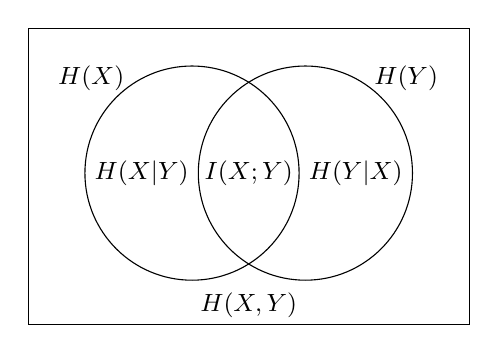
\begin{tikzpicture}[scale=0.8]
    \small
    % Labels
    \draw (0,0) node {$I(X;Y)$};
    \draw (-2.5,1.5) node {$H(X)$};
    \draw (2.5,1.5) node {$H(Y)$};
    \draw (-1.7,0) node {$H(X|Y)$};
    \draw (1.7,0) node {$H(Y|X)$};
    \draw (0,-2.1) node {$H(X,Y)$};
    % Circles
    \draw (-0.9,0) circle (1.7cm);
    \draw (0.9,0) circle (1.7cm);
    % Bounding Rectangle
    \draw (-3.5,-2.4) rectangle (3.5,2.3);
  \end{tikzpicture}
  \caption{Venn Diagram of Information-Theoretic Quantities}%
  \label{fig:venn-information}
\end{figure}

\subsection{Information-Theoretic View of GANs}%
\label{sec:info-value-function}%

We can now write a bit more about $\V = \mathbb{E}_{x \sim \pt}[{\log
  D_\theta(x)}] + \mathbb{E}_{z \sim \pz}[\log{(1 - D_\theta(G_\phi(z)))}]$ from
the perspective of information theory. The proposition presented below does not
consider the limiting behaviour of $D$ and $G$. Rather, we consider the
behaviour at each step of the algorithm. Section~\ref{sec:optimization-dynamics}
considers the limiting behaviour of the dynamics between $D$ and $G$.

We claim that the goal of GAN training is to minimize the Kullback-Leibler
divergence of the target probability distribution $\pt$ over the data and the
distribution of mass the discriminator $\D$ assigns to these data points.
Additionally, GAN training also maximizes the Kullback-Leibler divergence of the
generator's prior probability distribution $\pz$ and the distribution of mass
the discriminator assigns to synthetic data points $\D(\G(z))$. Lastly, GAN
training minimizes the Kullback-Leibler divergence of the generator's prior
distribution $\pz$ and the amount of mass the discriminator $\D(\G(z))$ assigns
to synthetic data points.

\begin{remark}
  The Kullback-Leibler divergence in this context can be thought of as how much
  more surprised we will be by outcomes drawn from $(\&X, p)$ since we are using
  an approximation $q$ of the true probability distribution $p$ over the set
  $\&X$.
\end{remark}

\begin{proposition}%
  \label{thm:info-objective}%
  If we consider
  \begin{align}
    \label{eq:consider}
    \min_\phi \max_\theta \mathbb{E}_{x \sim \pt}[{\log D_\theta(x)}] + \mathbb{E}_{z
    \sim \pz}[\log{(1 - D_\theta(G_\phi(z)))}]
  \end{align}
  from an information theoretic perspective, we can infer the training
  objectives of the GAN algorithm are to find
\begin{enumerate}[(i)]
  \item $\theta \in \Theta$ to minimize $\KL{\ptx}{\D(x)}$ and
    maximize $\KL{\pzz}{\D(\G(z))}$;
  \item $\phi \in \Phi$ to minimize $\KL{\pzz}{\D(\G(z))}$.
  \end{enumerate}
\end{proposition}

\begin{proof}
  The first term of $\V$ is the negative cross entropy of $\pt$ and
  the distribution induced by $\D(x)$,
\begin{align}
  \label{eq:neg-cross-entropy}
  - \&H(\pt, \D) = \sum_{x \in \&X}\ptx\log(\D(x)) = \mathbb{E}_{x \sim \pt} \left[\log(\D(x))\right].
\end{align}
Since we train the discriminator to maximize
(\ref{eq:neg-cross-entropy}) we can think of this as minimizing its
negative, which is equivalent to minimizing the cross entropy of $\pt$
and the distribution induced by $\D(x)$, which occurs when the
Kullback-Leibler divergence of $\pt$ and $\pd$ is 0, since
\begin{align}
  \&H(\pt,\D) & = - \sum_{x \in \&X} \ptx \log \pd \\
                   & = -\sum_{x \in \&X} \ptx \log \ptx + \sum_{x \in \&X} \ptx \log \ptx - \sum_{x \in \&X} \ptx \log \pd \\
                   & = -\sum_{x \in \&X} \ptx \log \ptx + \sum_{x \in \&X} \ptx \log {\ptx \over
                     \pd}  \\
                   & = H(\pt) + \KL{\pt}{\D}.
\end{align}
Since we do not touch $\pt$ during training, the only way to minimize
$\&H(\pt,\D)$ is to train $\D$ to minimize $\KL{\pt}{\D}$, which occurs when
$\pt = \D$. Therefore, when $\D$ has been optimized, $\D(x)$ will return the
probability that $x$ was sampled from $\pt$, which equals $\pt$ when $\D$ is
optimal. The second term of (\ref{eq:consider}),
\begin{align}
  \mathbb{E}_{z \sim \pz}\left[\log(1 - \D(\G(z)))\right] =
  \sum_{z \sim \pz} \pzz \log (1 - \D(\G(z)))
\end{align}
was maximized by $\D$, which is equivalent to $\D$ maximizing
\begin{align}
  -\sum_{z \sim \pz} \pzz \log (\D(\G(z))),
\end{align}
which is the cross entropy of $\pz$ and $\D(\G(z))$. This means $\D$ is trying
to make $\pz$ and $\D(\G(z))$ to be as different as possible. And given a fixed
discriminator $\D$, we train the $\G$ to minimize the same equation, which can
be expressed equivalently as minimizing
\begin{align}
  -\sum_{z \sim \pz} \pzz \log (\D(\G(z)))
\end{align}
the cross entropy of $\pz$ and $\D(\G(z))$.
\end{proof}

The interpretation of the above theorem is that the generator wants the
discriminator's decision on the generated data to be as uninformative as random
noise. The discriminator wants the distribution of its decision over the
training data to match the empirical probability distribution, while at the same
time, the discriminator wants its decision on the generated data to be more
informative than noise.

Next, we look at the optimization steps as the dynamics between approximating a
divergence and minimizing the same divergence.

\subsection{Optimization Dynamics}%
\label{sec:optimization-dynamics}

We discussed training $\D$ and $\G$ from the perspective of game theory in
Section~\ref{sec:derivation}. Now let us look at these results more rigorously
and with some actual calculations. Throughout this section, we will use the
following notation. Let $\&X$ be our data and $\pt$ the true probability
distribution over $\&X$. Let $\tilde{\&X}$ be the generated data and $\pg$ be
the distribution over $\tilde{\&X}$ induced by $\G$. Let $X$ be a random sample
from $(\&X, p^*)$, $\tilde{X}$ be a random sample from $(\tilde{\&X}, p_\phi)$,
and let $Z$ be a random sample from the prior probability space $(\&Z, \pz)$.

Throughout this section we will make use of not only
\begin{align}
  V(\phi, \theta)(X, Z) & = \sum_{x \in X}\pt\log{\D(x)} +
                          \sum_{z \in Z}\pz\log{(1 - \D(\G(z)))},
\end{align}
but of two equivalent variations as well. The first variation, $\tilde{V}(\phi,
\theta)(X, \tilde{X})$, is obtained by changing the second argument of $\V$ from
a sample of noise $Z$ to a sample from the generator $\G(Z) = \tilde{X}$. We
compute the second expectation with respect to $\pg$, i.e.\ we have
\begin{align}
  \tilde{V}(\phi, \theta)(X, \tilde{X}) = \sum_{x \in X}\ptx\log{\D(x)} + \sum_{\tilde{x} \in\tilde{X}}\pgx\log{(1 - \D(\tilde{x}))}.
\end{align}
For the second variation, $\&V$, we are going to embed our data into
$U \subset \R^2$, where each $u_i$ is associated with a pair
$(x_i, \tilde{x}_i)$. Then we can define the following function
\begin{align}
  \label{eq:joined}
  \Va(U) = \sum_{u \in U} \ptu \log \D(u) + \pgu \log(1 - \D(u)),
\end{align}
which we will use as short-hand for
\begin{align}
  \label{eq:joined-verbose}
  \sum_{u \in U} (p^* \circ \pi)(u)\log (\D \circ \pi)(u) + (\pg \circ \tilde{\pi})(u) \log(1 - (\D \circ \tilde{\pi})(u)),
\end{align}
where $\pi$ and $\tilde{\pi}$ are projections, i.e. $(f \circ \pi)(u) = (f
\circ \pi)((x, \tilde{x})) = f(x)$ and $(f \circ \tilde{\pi})(u) = (f
\circ \tilde{\pi})((x, \tilde{x})) = f(\tilde{x})$.

\begin{theorem}%
 \label{theorem:minimax}
 For any fixed $\G$, $\D$ maximizes $\V$ by playing its minimax
 decision rule and in doing so returns the following function
  \begin{align}
    \argmax_{\D}\V(\cdot) = \Dstar{\cdot}.
  \end{align}
\end{theorem}

\begin{proof}
  We compute the derivative of $\Va$ with respect to $\theta$,
  \begin{align}
    \label{eq:derivatives}
    {\partial \Va(U) \over \partial \theta} = \sum_{u \in U}\left[ \ptu { {\partial \D(u) \over \partial \theta} \over \D(u)} -
    \pgu {{\partial \D(u) \over \partial \theta} \over (1 - \D(u))}\right],
  \end{align}
  and when we let the derivative equal zero (looking only at the summand for
  clarity of notation) we can uncover $\D^*(u)$, by solving for $\D(u)$
  \begin{align}
    \label{eq:20}
    {\ptu \over \D(u)} = {\pgu \over (1 - \D(u))} \iff \D^*(u) = {\ptu \over \pgu + \ptu}.
  \end{align}
  Hence, for any fixed generator $G_\phi$, $\Va(U)$ is maximized when $\D$ takes
  the following action
  \begin{align}
    \label{eq:13}
    \D^*(u) = \Dstar{u}.
  \end{align}
  Hence $\argmax_{\D}\V(\cdot, \cdot) = \Dstar{\cdot}$.
\end{proof}

Now that we have the minimax decision rule, we can place it in the
value function $\tilde{V}$, to uncover
$\max_{\D}\tilde{V}(\phi, \theta)(X, \tilde{X})$, equal to
\begin{align}
  \label{eq:sum-of-two-kl-divergences}
   \mathbb{E}_{x \sim \pt}\left[\log{{\ptx \over p_{\phi}(x)+ \ptx}}\right] + \mathbb{E}_{\tilde{x} \sim \pg}\left[\log{\pgx \over \pgx + p^*(\tilde{x})} \right],
\end{align}
which is the sum of two Kullback-Leibler divergences (which is related
to the Jenson-Shannon divergence of $\pt$ and $\pg$)
i.e. $\max_{\D}\V(X, Z)$ is equal to
\begin{align}
  \label{eq:16}
  \KL{\pt}{p_{\phi} + \pt} + \KL{\pg}{\pg + p^*}.
\end{align}
\begin{lemma}
  The minimax value for $\D$, i.e. $\min_{\phi}\max_{\theta}\V(X, Z)$, is $ - \log{4}$.
\end{lemma}

\begin{proof}
  The training goal for $\G$ is to learn $\pt$, so the optimal $\G$ is $\G^* =
  \pt$. If this optimal $\G^*$ is place inside (\ref{eq:16}), we obtain
  \begin{align}
    \label{eq:side-note}
    V(\phi^*, \theta)(X, \tilde{X}) & = \sum_{x \in X}\ptx \log{\ptx \over 2 \ptx} + \sum_{\tilde{x} \in \tilde{X}}p^*(\tilde{x}) \log{ p^*(\tilde{x}) \over 2 p^*(\tilde{x})} \\
                      & = \sum_{x \in X} \ptx \log {1 \over 2} + \sum_{\tilde{x} \in \tilde{X}} p^*(\tilde{x}) \log {1 \over 2} \\
                      & = -\log{4}
  \end{align}
  Hence, the minimax value is $ - \log{4}$.
\end{proof}

\begin{theorem}%
  \label{thm:limiting}
  When $\D$ is optimal, minimizing $\V$ as a function of $\phi$ is equivalent to
  optimizing the Jensen-Shannon divergence.
\end{theorem}

\begin{proof}
  We can make the relationship between (\ref{eq:16}) and the
  Jensen-Shannon divergence by adding and subtracting $\log{4}$ from
  (\ref{eq:16}), which yields
  \begin{align}
    \label{eq:desired}
    V(\phi, \theta^*) = 2 \cdot \JSD{\pt}{\pg} - \log{4},
  \end{align}
  which is what we wanted. See Appendix~\ref{sec:proof-for-jsd-thing} for
  complete details.
\end{proof}

\subsection{Discussion}

% Theoretically, one reason that GANs are so successful is because
% they do not rely on traditional maximum likelihood methods, which
% are equivalent to minimizing the Kullback-Leibler divergence.

% To see this, let $p\left(x | \theta^{(*)}\right)$ be a probability
% distribution we wish to estimate and let
% $p\left(x | \theta^{\left(t\right)}\right)$ be our estimate at
% iteration $t$.  Then
% \begin{align}
%   \label{eq:equivalent-mle}
%   \KL{p\left(x | \theta^{(*)}\right)}{p\left(x | \theta^{\left(t\right)}\right)} =
%   H\left(p\left(x | \theta^{(*)}\right)\right) -
%   \mathbb{E}_{x \sim p\left(x | \theta\right)}\left[ \log p\left(x | \theta^{\left(t\right)}\right) \right],
%  \end{align}
% and minimizing the cross entropy term on the right is equivalent to maximizing
% \begin{align}
%   \mathbb{E}_{x \sim p\left(x | \theta\right)}\left[ \log p\left(x | \theta^{\left(t\right)}\right) \right].
% \end{align}
% Maximizing this term is equivalent to maximizing the likelihood
% function for $p\left(x | \theta\right)$.

% The discriminator's job is to classify data points as real or fake,
% which is equivalent to compression. The discriminator is optimized
% to cluster the data into two classes, real and fake. Neural networks
% are good at finding regularities in data and one way to express
% regularity is by clustering similar objects into groups.

This section included two information theoretic perspectives on GAN training.
Theorem~\ref{thm:limiting} considered the theoretical, limiting behaviour of
GANs and~\ref{thm:info-objective} considered what happens at each step of the
optimization.

As for Theorem~\ref{thm:limiting}, the measure that $G$ minimizes changes at
each training step since $D$ forces $\V$ into a better approximation of the
Jensen-Shannon divergence one step at a time by performing the actions
enumerated in Theorem~\ref{thm:info-objective}. It is useful to consider what
happens at each step of training. When we do that, we observe the generator and
discriminator minimizing and maximizing the Kullback-Leibler divergence to
optimize the fit of $D$ and $G$ to $(\&X, \pt)$.

%%% Local Variables:
%%% mode: latex
%%% TeX-master: "../thesis.tex"
%%% End:
